\FloatBarrier

\myworries{//20191123 esta rodando no pc da lu}

A simulação para o modelo de \textit{trapping-detrapping} explicado na Seção \ref{sec:my-trapdetrap} com concentração da superfície constante, ou seja $N(0,t)=C_{eq}$ (similar à condição de contorno para nitretação gasosa da Seção \ref{sec:trap-detrap-gas-cc}), utilizou os parâmetros mencionados na Seção \ref{params_sub}, a concentração de equilíbrio definida na Seção \ref{sec:ceq-param}, temperatura de 673K e os seguinte valores para a aplicação do método numérico:$\Delta t$ e $\Delta x$ utilizados foram 0,0001s e 0,1 $\mu m$, para um tempo total de 22 horas e 20 $\mu m$ de profundidade.

Os resultados dessa simulação estão representados nas Figuras \ref{fig:td-cscte1} e \ref{fig:td-cscte-both}, a primeira mostra o desenvolvimento do perfil de concentração de nitrogênio no tempo e a segunda mostra o perfil de concentração de nitrogênio livre, aprisionado e total após 2 horas.

\begin{figure}[ht]
\centering
	\caption{Resultado da simulação para o modelo de \textit{trapping-detrapping} para concentração na superfície constante, até 2 horas}
	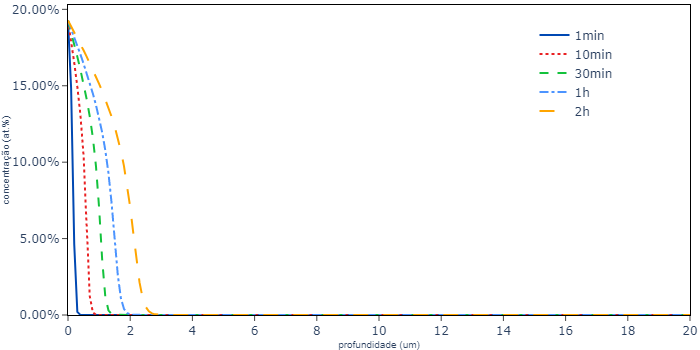
\includegraphics[width=1.0\textwidth]{plot_TrapDetrapCte}
	\label{fig:td-cscte1}
	\centering
	\fonte{Elaborado pela autora}
\end{figure}


\begin{figure}[ht]
\centering
	\caption{Resultado da simulação para o modelo de \textit{trapping-detrapping} para concentração na superfície constante - Perfil de Concentração de nitrogênio Livre e Aprisionado, após 2 horas }
	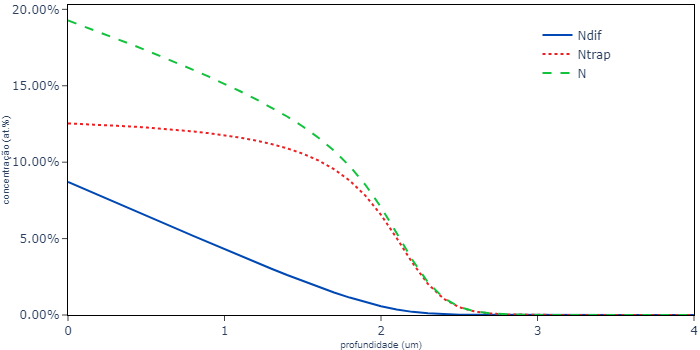
\includegraphics[width=1.0\textwidth]{plot_TrapDetrapCteBoth2h}
	\label{fig:td-cscte-both}
	\centering
	\fonte{Elaborado pela autora}
\end{figure}

Na Figura \ref{fig:td-cscte-compara}, foram plotadas ambas as soluções dos dois modelos estudados, para concentração da superfície constante, mostrando o perfil de concentração de nitrogênio após 2 horas obtido para cada um.

\begin{figure}[ht]
\centering
	\caption{Resultado da simulação para os dois modelos com concentração superficial constante, após 2 horas }
	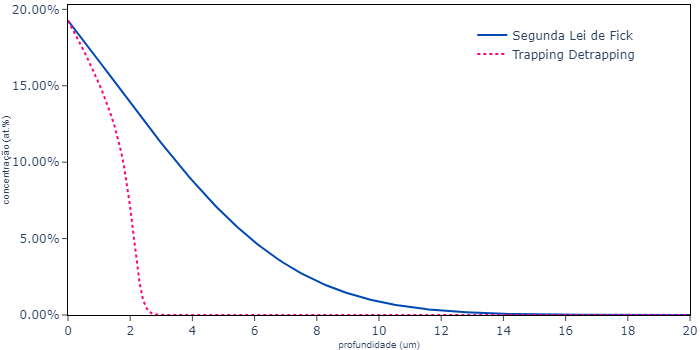
\includegraphics[width=1.0\textwidth]{plot_AmbosCsCte2h}
	\label{fig:td-cscte-compara}
	\centering
	\fonte{Elaborado pela autora}
\end{figure}
\FloatBarrier

